% Author: Noel Dawe

\documentclass[11pt]{article}

\usepackage[margin=1in]{geometry}

\usepackage{graphicx}
\usepackage[usenames,dvipsnames,svgnames,table]{xcolor}
\usepackage{mathrsfs}
\usepackage{amssymb,amsmath}


\usepackage{tikz,pgfplots,tikz-3dplot}
%\pgfplotsset{compat=1.9}
\usepackage{tikzscale}
\usepackage{environ}
\usepackage[outline]{contour}
\contourlength{2pt}

% scale a tikz figure to \textwidth
% http://tex.stackexchange.com/questions/6388/how-to-scale-a-tikzpicture-to-textwidth
\makeatletter
\newsavebox{\measure@tikzpicture}
\NewEnviron{scaletikzpicturetowidth}[1]{%
  \def\tikz@width{#1}%
  \def\tikzscale{1}\begin{lrbox}{\measure@tikzpicture}%
  \BODY
  \end{lrbox}%
  \pgfmathparse{#1/\wd\measure@tikzpicture}%
  \edef\tikzscale{\pgfmathresult}%
  \BODY
}
\makeatother

\usetikzlibrary{arrows}
\usetikzlibrary{snakes}
\usetikzlibrary{shapes}
\usetikzlibrary{shadows}
\usetikzlibrary{trees}
\usetikzlibrary{arrows}
\usetikzlibrary{positioning}                % For "above of=" commands
\usetikzlibrary{calc,through}               % For coordinates
\usetikzlibrary{decorations.pathreplacing}  % For curly braces
\usetikzlibrary{calc}
\usetikzlibrary{fadings}

% http://www.math.ucla.edu/~getreuer/tikz.html
\usepackage{pgffor}                         % For repeating patterns

% Define the layers to draw the diagram
\pgfdeclarelayer{background}
\pgfdeclarelayer{foreground}
\pgfsetlayers{background,main,foreground}


\begin{document}

The helical path of a track is parametrized at the point of closest approach
to the z-axis of the detector coordinate system or the z-axis of a coordinate
system centered at a vertex. The \emph{perigee parameters}
$(d_0, z_0, \phi_0, \theta, \frac{q}{p})$ are illustrated in
Figure~\ref{fig:perigee} and are defined as follows:

\begin{itemize}
\item $d_0$: The transverse impact parameter is the distance of closest
    approach to the z-axis in the $x-y$ plane. The sign of $d_0$ is
    positive when $\phi - \phi_0 = \frac{\pi}{2} \mod 2\pi$.
\item $z_0$: The longitudinal impact parameter is the z-coordinate at the
    perigee.
\item $\phi_0$: The azimuth angle of the track at the perigee, measured in
    the range $[-\pi, \pi]$.
\item $\theta$: The polar angle of the track, measured in the
    range $[0, \pi]$.
\item $\frac{q}{p}$: The ratio of the track charge to the magnitude of the
    track momentum.
\end{itemize}

\begin{figure}[h]
\centering
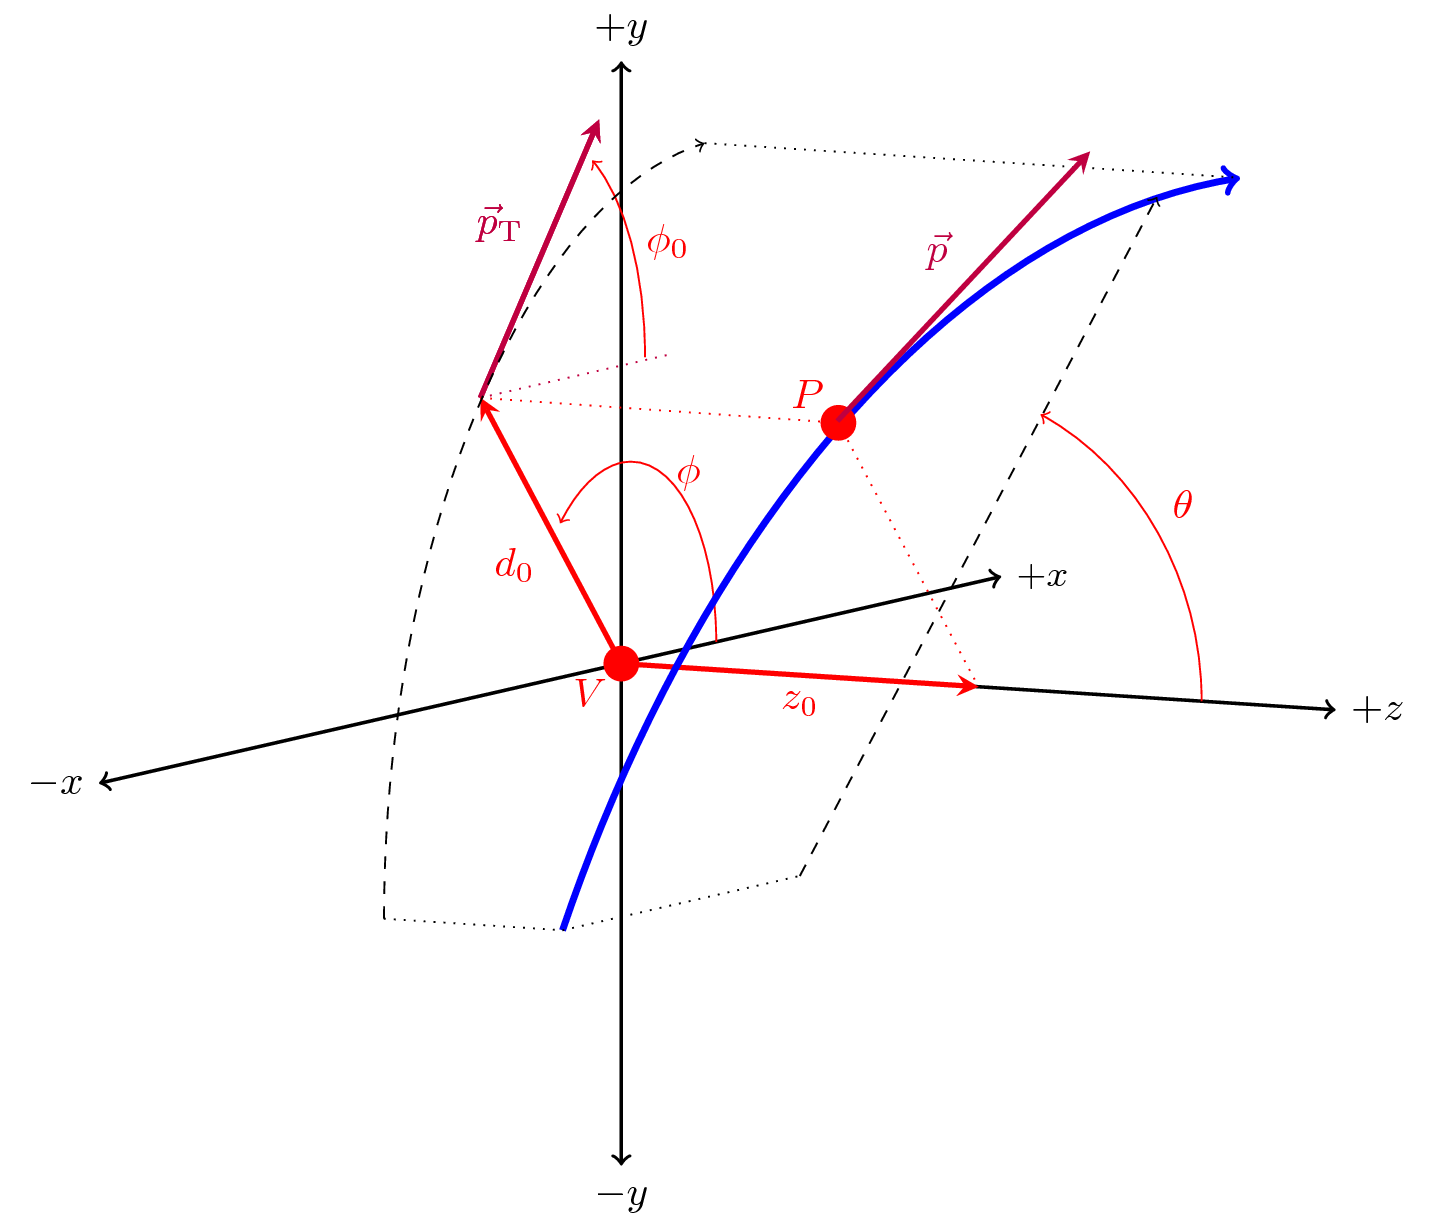
\includegraphics[width=0.8\textwidth]{perigee.tikz}
\caption{
Illustration of the perigee parameters of the point of closest approach $P$ of
a track (blue curve) to the z-axis of a coordinate system centered at vertex $V$.
The projections of the track onto the $x-y$ and $y-z$ planes are shown
with the dashed black paths.}
\label{fig:perigee}
\end{figure}

\end{document}
